%!TEX root = met-top-spaces.tex
\stepcounter{lecture}
\setcounter{lecture}{3}
\sektion{Connectedness}

\subsection{Basic notions} % (fold)
\label{sub:basic_notions}

\begin{definition}
	A topological space $X$ is \emph{disconnected} if there are non-empty open subsets $U, V$ with $U\cap V = \emptyset$ and $X=U\cup V$. Otherwise $X$ is called \emph{connected}.

	In other words, $X$ is connected if and only if, given open sets $U,V$ with $U \cap V = \emptyset$ and $X=U\cup V$, either $U=\emptyset$ or $V=\emptyset$ (equivalently, either $U=X$ or $V=X$).
\end{definition}

Clearly connectedness is a topological property. We can extend this definition to subsets:

\begin{definition}
	If $Y$ is a subset of the topological space $X$, then $Y$ is disconnected in the subspace topology if and only if there are $U, V$ open in $X$ such that $U\cap V=\emptyset$, $V\cap Y\neq \emptyset$ but $U\cap V\cap Y=\emptyset$ and $Y\subset U\cup V$. In this case, we say that $U$ and $V$ \emph{disconnect} $Y$.
\end{definition}

\begin{proposition}
	Let $X$ be a topological space. Then the following are equivalent: \label{prop:equivalent-properties}
	\begin{enumerate}
		\shortskip
		\item $X$ is connected;
		\item The only subsets of $X$ that are both open and closed are $\emptyset$ and $X$;
		\item Every continuous function $f:X\to\Z$ is constant.
	\end{enumerate}
\end{proposition}

\begin{proof}
	$\text{(i)} \iff \text{(ii)}$ is trivial, since for $U\subset X$, we consider that $U \cup (X\backslash U) = X$.

	$\text{(i)} \implies \text{(iii)}$. Suppose there is a non-constant map $f:X\to\Z$, then there exists $m<n$ such that both $m,n$ are in $f(X)$. Then $f^{-1}(\{k:k\leq m\})$ and $f^{-1}(\{k:k>m\})$ are open, non-empty sets disconnecting $X$; that is, $X$ is \emph{not} connected.

	$\text{(iii)} \implies \text{(i)}$. Suppose that $X$ is not connected; that is, there are non-empty, disjoint open $U$, $V$ such that $X=U\cup V$. Consider the map $f:X\to\Z$ defined by %
	\begin{equation*}
		f(x) =
		\begin{cases}
			0 & \text{if } x\in U, \\ %
			1 & \text{if } x\in V.
		\end{cases}
	\end{equation*}
	This is continuous (even locally constant) function, but not globally constant.
\end{proof}

\begin{proposition}
	A continuous image of a connected space is connected.
\end{proposition}

\begin{proof}
	If $f:X\to Y$ is a surjective continuous map of topological spaces and if $U, V$ disconnect $Y$, then their pre-images $f^{-1}(U), f^{-1}(V)$ disconnect $X$. Thus, if $X$ is connected, then so is $Y$.
\end{proof}

	\pagebreak

\subsubsection*{Connectedness in R} % (fold)
\label{ssub:connectedness_in_r}

\vspace{9pt}

\begin{definition}
	A set $I\subseteq \R$ is called an \emph{interval} if, given $x,z\in I$ with $x\leq z$, we have $y \in I$ for all $y$ such that $x\leq y\leq z$.

	We have the cases $\inf I=a\iR$ and $a\in I$, or $a\not\in I$, or $\inf I = -\infty$. Similarly, we have the cases $\sup I=b\iR$ and $b\in I$, or $b\not\in I$, or $\sup I = \infty$. Thus any interval $I$ takes the form $[a,b]$, $[a,b)$, $(a,b]$, $[a,\infty)$, $(a,\infty)$, $(-\infty,b]$, $(-\infty,b)$ or $(-\infty,\infty)$.
\end{definition}

\begin{theorem}
	A subset of $\R$ is connected if and only if it is an interval. \label{thm:cnncted-R-interval}
\end{theorem}

\begin{proof}
	First suppose that $X\subseteq\R$ is not an interval. Then we can find $x<y<z$ with $x,z\in X$ but $y\not\in X$. Then $(-\infty,y)$ and $(y,\infty)$ disconnect $X$.

	Now suppose that $I$ is an interval, and $I\subseteq U \cup V$, where $U,V$ are open subsets of $\R$ disconnecting $I$. Then there exists $u\in U\cap I$, $v\in V\cap I$ where, without loss of generality, $u<v$. Since $I$ is an interval, $[u,v] \subseteq I$. Let $s=\sup[u,v] \cap U$.

	If $s\in U$, then $s<v$, so $s\neq v$. As $U$ is open, there is $\delta>0$ with $(s-\delta,s+\delta) \subset U$. Hence there is $s\p \in [u,v]\cap U$ with $s\p>s$, contradicting $s$ as an upper bound.

	If $s\in V$, then there exists $\delta$ such that $(s-\delta,s+\delta) \subset V$. Then $(s-\delta,s+\delta) \cap U = \emptyset$ implies $[u,v] \cap U \subset [u,s-\delta]$, which contradicts $s$ as a \emph{least} upper bound. Thus $I$ is connected.
\end{proof}

\begin{corollary}
	[Intermediate value theorem] Let $a<b$ and $f:[a,b]\to\R$ be a continuous function. If $y\in[f(a),f(b)]$ (or $[f(b)],f(a)]$ as appropriate), then there exists $x\in [a,b]$ such that $f(x)=y$.
\end{corollary}

\begin{proof}
	If not, then $f^{-1}((-\infty,y))$ and $f^{-1}((y,\infty))$ disconnect $[a,b]$.
\end{proof}

% subsubsection connectedness_in_r (end)

\subsubsection*{Connected subsets and subspaces} % (fold)
\label{ssub:connected_subsets_and_subspaces}

\begin{proposition}
	Let $\{Y_\alpha\}_{\alpha\in A}$ be connected subsets of a topological space $X$, such that $Y_\alpha \cap Y_\beta \neq \emptyset$ for all $\alpha,\beta \in A$. Then their union $Y=\bigcup_{\alpha\in A} Y_\alpha$ is connected. \label{prop:connected-unions}
\end{proposition}

\begin{proof}
	Use proposition~\ref{prop:equivalent-properties}: we wish to prove that any continuous function $f:Y\to\Z$ is constant. Now, the restriction $f_\alpha = \eval[1]{f}_{Y_\alpha}$ is constant on $Y_\alpha$, for all $\alpha$; say, $f_\alpha(x)=n_\alpha$ for $x\in Y_\alpha$.
	% 
	Then for all $\beta\neq \alpha$, there exists $z\in Y_\alpha \cap Y_\beta$, and we have $n_\alpha = f(z) = n_\beta$. Thus $f$ is constant on $Y$.
\end{proof}

\begin{definition}
	A \emph{connected component} of a topological space $X$ is a \emph{maximal} conected subset $Y$; that is, if $Z\subseteq X$ is connected and $Z\supseteq Y$, then $Z=Y$.
	
	Each point $x\in X$ is contained in a unique connected component of $X$, namely $\bigcup\{Z \text{ connected subset of } X \text{ with } x\in Z\}$. This is connected by proposition~\ref{prop:connected-unions}, since $x\in Z$ for each $Z$, and clearly it's maximal.
\end{definition}

\begin{example}
	Take $X=\{0\} \cup \{1/n: n=1,2,3,\ldots\}$, with the subspace topology. The connected component containing $1/n$ is clearly just $\{1/n\}$, both open and closed in $X$. The component containing $0$ is $\{0\}$, which is closed but not open.
\end{example}

	\pagebreak

\begin{proposition}
	If $Y$ is a connected subset of a topological space $X$, then the closure $\closure{Y}$ is connected.
\end{proposition}

\begin{proof}
	Suppose $f:\closure{Y}\to\Z$ is continuous. Then proposition~\ref{prop:equivalent-properties} tells us that $\eval[0]{f}_Y$ is constant; say $f(y)=m$ for all $y\in Y$. Then given any $x\in\closure{Y}$, let $f(x)=n$; then $f^{-1}(n)$ is an open neighbourhood of $x$ in $Y$; that is, of the form $U\cap\closure{Y}$ with $U$ open in $X$.
	
	Since $x\in\closure{Y}$, this contains a point of $Y$ (where $f$ takes the value $m$), so $n=m$, and hence $f$ is constant on $\closure{Y}$. Hence $\closure{Y}$ is connected.
\end{proof}

\vspace{3pt}

\begin{remark}
	Thus connected components of a space are always closed (since they are a \emph{maximal} connected subset), but as in the above example, not necessarily open.
\end{remark}

\begin{definition}
	We call a space $X$ \emph{totally disconnected} if its only connected components are single points; that is, its only connected subsets are single points.
\end{definition}

Any discrete topological space is totally disconnected, as was the previous example.

\begin{lemma}
	If $X$ is a topological space and for all $x,y\in X$ with $x\neq y$, $X$ may be disconnected by $U,V\subseteq X$, where $x\in U$ and $y\in V$, then $X$ is totally disconnected. \label{lem:trivial}
\end{lemma}

\begin{proof}
	For any subset $Y$ with points $x\neq y$, then for $U$ and $V$ as above, $U\cap Y$ and $V\cap Y$ disconnect $Y$. %
\end{proof}

The irrationals $\R\backslash\Q$ are totally disconnected: use the above lemma, and the fact that the rationals are dense in the irrationals.

% subsubsection connected_subsets_and_subspaces (end)

\subsubsection*{The Cantor set} % (fold)
\label{ssub:the_cantor_set}

We start with $I_0=[0,1]$, and remove $(\f{1}{3},\f{2}{3})$ to obtain $I_1 = [0,\f{1}{3}] \cup [\f{2}{3},1]$. We then remove the middle third from both $[0,\f{1}{3}]$ and $[\f{2}{3},1]$ to obtain $I_2$. Proceed recursively:

\begin{center}
	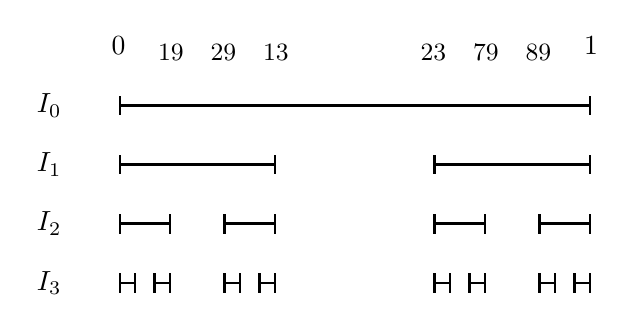
\begin{tikzpicture}[xscale=6]
		
		\foreach \s in {0,1} {\draw (\s,0.45) node [above=2pt] {$\s$};}
		\foreach \s in {1,2} {\draw (\s/3,0.45) node [above] {\small{$\f{\s}{3}$}};}
		\foreach \s in {1,2,7,8} {\draw (\s/9,0.45) node [above] {\small{$\f{\s}{9}$}};}

		\foreach \s in {0,...,3} {\draw (-0.1,-\s*0.75) node [left] {$I_\s$};}

		% I_0
		\foreach \s/\t in {0/1} {\draw [thick, |-|] (\s,0) -- (\t,0);}

		% I_1
		\foreach \s/\t in {0/1, 2/3} {\draw [thick, |-|] (\s/3,-0.75) -- (\t/3,-0.75);}

		% I_2
		\foreach \s/\t in {0/1, 2/3, 6/7, 8/9} {\draw [thick, |-|] (\s/9,-1.5) -- (\t/9,-1.5);}

		% I_3
		\foreach \s/\t in {0/1, 2/3, 6/7, 8/9, 18/19, 20/21, 24/25, 26/27} {\draw [thick, |-|] (\s/27,-2.25) -- (\t/27,-2.25);}

		% % I_4
		% \foreach \s/\t in {0/1, 2/3, 6/7, 8/9, 18/19, 20/21, 24/25, 26/27, 54/55, 56/57, 60/61, 62/63, 72/73, 74/75, 78/79, 80/81}
		% {
		% 	\draw [thick] (\s/81,-3) -- (\t/81,-3);
		% }
	\end{tikzpicture}
\end{center}

and so on. Then the \emph{Cantor set $C$} is given by
\begin{equation*}
	C = \bigcap_{n\geq 0} I_n.
\end{equation*}
We can understand this in terms of ternary (base~3) expansions; that is, expansions of the form $0\cdot a_1 a_2 a_3\ldots$, where each $a_i = 0,1,2$. Without loss of generality, we impose $1/3=0.022\ldots$.

Then $I_1$ consists of numbers with $a_1=0$ or $2$. Then $I_2$ has $a_1=0$ or $2$, and $a_2=0$ or $2$, and so on for $I_3$. Thus $C$ consists of numbers with a ternary expansion where each $a_i = 0$ or $2$.

Suppose now we are given two points $x,y\in C$ with $x\neq y$. For some $n$, the ternary expansions will differ in the $n$th place (and without loss of generality, they are the same in all previous places). Now $C \subset I_n$, which consists of $2^n$ closed intervals, one of which contains $x$, and one of which contains $y$.

Then we can disconnect $I_n$ by open $U,V$, where $U \cap V = \emptyset$, $x\in U$ and $y\in V$. Then $C=(U \cap C) \cup (V \cap C)$, and $x\in U \cap C$, $y\in V\cap C$. Then lemma~\ref{lem:trivial} tells us that $C$ is totally disconnected.

Note that both $C$ and its complement are uncountable (clear from the ternary expansion).

% subsubsection the_cantor_set (end)

% subsection basic_notions (end)

\subsection{Path connectedness} % (fold)
\label{sub:path_connectedness}

\begin{definition}
	Let $X$ be a topological space and $x,y\in X$. A \emph{path} from $x$ to $y$ is a continuous function $\phi:[a,b]\to X$ such that $\phi(a)=x$, $\phi(b)=y)$ (We sometimes take take $a=0$, $b=1$.)
	
	$X$ is \emph{path-connected} if, for all $x,y\in X$, there is a path from $x$ to $y$.
\end{definition}

\begin{proposition}
	The continuous image of a path-connected space is path-connected.
\end{proposition}

\begin{proof}
	Suppose $X$ is path-connected and $f:X\to Y$ is a continuous surjection. Given $y_1,y_2\in Y$, choose $x_i\in f^{-1}_i(y_i)$, $i=1,2$ and a path $\gamma:[a,b]\to X$ from $x_1$ to $x_2$. Then there is a path $f\circ\gamma:[a,b]\to Y$ from $y_1$ to $y_2$.
\end{proof}

\begin{proposition}
	Path connectedness implies connectedness. \label{prop:path-connected-implies}
\end{proposition}

\begin{proof}
	Suppose $X$ is a topological space and $X=U\cup V$, with $U, V$ disconnecting $X$. Suppose for contradiction that $X$ is not path-connected. If it were, then choose $u\in U$, $v\in V$, and there is a continuous function $\phi:[a,b]\to X$ such that $\phi(a)=u$, $\phi(b)=v$. Then $\phi^{-1}(U)$ and $\phi^{-1}(V)$ are non-empty open subsets of $[a,b]$ which disconnect $[a,b]$.
\end{proof}

Note that the converse is false: connectedness does not imply path connectedness, as the following example shows:

\begin{example}
	In $\R^2$, first define
	\begin{equation*}
		I = \left\{(x,0) : 0<x\leq 1\right\}
		\qqand
		J = \left\{(0,y) : 0<y\leq 1\right\}.
	\end{equation*}
	Then for $n=1,2,\ldots$, define
	\begin{equation*}
		L_n = \left\{(1/n,y): 0\leq y\leq 1\right\}.
	\end{equation*}
	Now set $X=I \cup J \cup \left( \bigcup_{n\geq 1} L_n \right)$ with the subspace topology.

	\begin{center}
		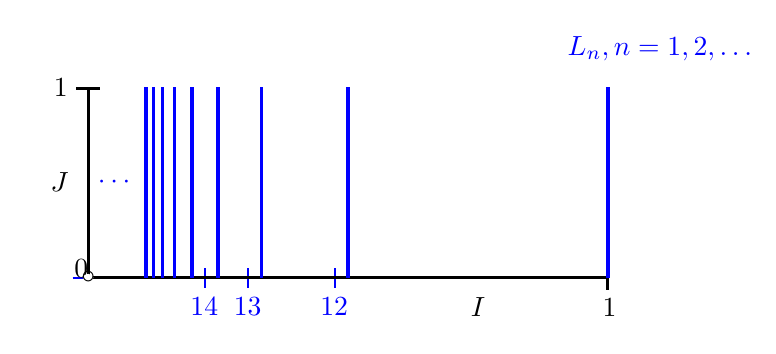
\begin{tikzpicture}[xscale=3,scale=2.2,yscale=1.1]
			
			\foreach \s in {2,3,4} {
				\draw [thick, -|, blue] (-0.003,0) -- (1/\s+0.003,0);
				\draw [blue] (1/\s,0) node [below=3.5pt] {$\f{1}{\s}$};
			}

			\bigarrow (0,0) node [below left] {$0$} -- (1.2,0);
			\bigarrow (0,0) -- (0,1.2);

			\draw [very thick, -|] (-0.003,0) -- (1.003,0) node [below=3.5pt] {$1$};
			\draw [very thick, -|] (0,-0.009) -- (0,1) node [left=3.5pt] {$1$};

			\draw (0.75,0) node [below=3.5pt] {$I$};
			\draw (0,0.5) node [left=3.5pt] {$J$};

			\draw [blue] (0,0.5) node [right] {$\cdots$};

			\foreach \s in {1,...,9} {\draw [very thick, blue] (1/\s,0) -- (1/\s,1);}

			\draw [blue] (1.1,1.2) node {$L_n, n=1,2,\ldots$};

			\fill [white] (0,0) circle (0.01 and 0.02);
			\draw (0,0) node {$\circ$};
		\end{tikzpicture}
	\end{center}

	It is easy to see that $X$ is not path-connected: for any continuous path $\gamma(t) = (\gamma_1(t), \gamma_2(t))$ from $(1,0)$ to $(0,1)$, there is some $s$ such that $\gamma_1(s)=0$ and $\gamma_1(t)>0$ for all $t<s$, so we must also have $\gamma_2(s)=0$. This means that $\gamma$ passes through $(0,0)$, but this is not in $X$.

	However, such an $X$ is connected. Suppose $f:X\to\Z$ is a continuous function. Then $f$ is constant on $J$ and on $Y=I \cup \left( \bigcup_{n\geq 1} L_n \right)$. However, the points $(1/n,1/2) \in Y$ have limit $(0,1/2) \in J$ as $n\to\infty$, and by the continuity of $f$, the two constants agree. Thus $f$ is constant on $X$.
\end{example}

Given a topological space $X$, we can define an equivalence relation $\sim$ on $X$ by $x\sim y$ if and only if there is a path from $x$ to $y$ in $X$. This is indeed an equivalence relation:
\begin{itemize}
	\shortskip
	\item Reflexivity: $x\sim x$ is trivial.
	\item Symmetry: if $\phi:[a,b] \to X$ is a path from $x$ to $y$, then $\psi(t) = \phi(-t)$ gives a path $\psi:[-b,-a] \to X$ from $y$ to $x$.
	\item Transitivity: suppose $x\sim y$ and $y\sim z$. Then there are paths $\phi:[a,b] \to X$ and $\psi:[c,d] \to X$ with $\phi(a)=x$, $\phi(b) = y = \psi(c)$ and $\psi(d)=z$. So define a new path $\chi:[a,b+d-c] \to X$ by
	\begin{equation*}
		\chi(t) =
		\begin{cases}
			\phi(t) & a\leq t\leq b, \\ %
			\psi(t+c-b) & b\leq t\leq b+d-c.
		\end{cases}
	\end{equation*}
	Then $\chi$ is continuous at all points $t\in[a,b+d-c]$ (which is easy to check), and it gives a path from $x$ to $z$. Thus $x\sim z$.
\end{itemize}

\begin{definition}
	The equivalence classes of $\sim$ are called the \emph{path-connected components} of $X$.
\end{definition}

\begin{theorem}
	Let $X$ be an open subset of Euclidean space $\Rn$. Then $X$ is connected if and only if $X$ is path connected.
\end{theorem}

\begin{proof}
	Path-connectedness implies connectedness by proposition~\ref{prop:path-connected-implies}.

	Now the converse: suppose $X$ is connected and $x\in X$. Let $U$ be the equivalence class of $x$ under the equivalence relation $\sim$ defined above.

	Now, $U$ is open in $X$: suppose $y\in U$, whence $x \sim y$. Since $X$ is open, there exists $\delta>0$ such that $B(y,\delta) \subseteq X$. Then for all $z\in B(y,\delta)$, we have $y\sim z$, by taking the straight line segment. Transitivity implies that $x\sim z$ for all $z\in B(y,\delta)$, and thus $B(y,\delta) \subset U$, and $U$ is open.

	Similarly, $X\backslash U$ is open. Suppose $y\in X\backslash U$. Since $X$ is open, there exists $\delta>0$ such that $B(y,\delta) \subseteq X$. For $z\in B(y,\delta)$, we have $y\sim z$ as above, and then $x \not\sim z$, hence $B(y,\delta) \subsetneq X\backslash U$.

	Since $X$ is connected, we must have $X\backslash U=\emptyset$ and $U=X$. Hence $X$ is path-connected, since $x\sim y$ for all $y\in X$.
\end{proof}

% subsection path_connectedness (end)

	\pagebreak

\subsection{Products of connected spaces} % (fold)
\label{sub:products_of_connected_spaces}

\begin{proposition}
	\label{prop:3-path-connected-product-topology}
	Let $X$ and $Y$ be topological spaces. If $X$ and $Y$ are path-connected, then so too is $X\times Y$, with the product topology.
\end{proposition}

\begin{proof}
	Given $(x_1,y_1)$ and $(x_2,y_2)\in X\times Y$, we know that there are paths $\gamma_1:[0,1]\to X$ and $\gamma_2:[0,1]\to Y$ with $\gamma_1(0)=x_1$, $\gamma_1(1)=x_2$, $\gamma_2(0)=y_1$ and $\gamma_2(1)=y_2$.
	
	Now define a map $\gamma:[0,1]\to X\times Y$ by $\gamma(t) = (\gamma_1(t),\gamma_2(t))$. % We claim that this $\gamma$ is continuous.
	% 
	The base for the topology on $X\times Y$ consists of the open sets $U\times V$, with $U$ open in $X$ and $V$ open in $Y$. So it is sufficient to prove that $\gamma^{-1}(U\times V)$ us open for all such $U$ and $V$. But $\gamma^{-1}(U\times V)=\gamma^{-1}(U) \cap \gamma^{-1}(V)$ is clearly open. So $\gamma$ is continuous and defines a path from $(x_1,y_1)$ to $(x_2,y_2)$.
\end{proof}

\begin{proposition}
	If $X$ and $Y$ are connected, then so too is $X \times Y$ with the product topology. \label{prop:connected-products}
\end{proposition}

\vspace{-8pt}

First we make some general comments about product topologies. Given $y\in Y$, the set $X\times\{y\}$ with the subspace topology is homeomorphic to $X$, using the projection map $\pi_1:X \times \{y\} \to X$. We already know that this map is a continuous bijection.

However, a base for the topology on $X \times Y$ consists of open sets $U\times V$, with $U$ open in $X$ and $V$ open in $Y$. This implies that a base for the subspace topology on $X\times\{y\}$ consists of subsets $U\times\{y\}$, for $U$ open subsets of $X$. Thus, under $\eval[0]{\pi_1}_{X\times\{y\}}$, open sets do correspond, and hence $\pi_1:X\times \{y\} \to X$ is a homeomorphism.

Similarly, for $x\in X$, $\{x\} \times X$ is homeomorphic to $Y$, and so $X \times \{y\}$ is connected for all $y\in Y$. Thus $\{x\} \times X$ is connected for all $x\in X$.

\begin{proof}
	[Proof of proposition~\ref{prop:connected-products}] Given a continuous function $f:X \times Y \to \Z$, it is obvious that $f$ is constant on each slice $\{x\} \times Y$ and $X \times \{y\}$, by connectedness.

	\begin{center}
		\begin{tikzpicture}
			
			\bigarrow (0,0) -- (4.5,0) node [below=2pt] {$X$};
			\bigarrow (0,0) -- (0,4.5) node [left=2pt] {$Y$};

			\foreach \s in {1,2} {
				\draw [dashed] (\s*1.5,0) node [below=3pt] {$x_\s$} -- (\s*1.5,4.2);
				\draw [dashed] (0,\s*1.5) node [left=2pt] {$y_\s$} -- (4.2,\s*1.5);
				\draw (\s*1.5,\s*1.5) node {$\bullet$};
			}

			\draw (1.5,1.5) node [below left] {$(x_1,y_1)$};
			\draw (3,3) node [above right] {$(x_2,y_2)$};

			\draw (0,0) node [below left=2pt] {$0$};
		\end{tikzpicture}
	\end{center}

	Given arbitary points $(x_1,y_1), (x_2,y_2) \in X\times Y$, we deduce that $f(x_1,y_1) = f(x_1,y_2) = f(x_2,y_2)$ (see diagram). Hence $f$ is constant on $X\times Y$ and $X\times Y$ is connected.
\end{proof}

\vspace{3pt}

\begin{remark}
	A similar argument also proves proposition \ref{prop:3-path-connected-product-topology}: there is a path joining $(x_1,y_1)$ to $(x_1,y_2)$ and a path joining $(x_1,y_2)$ to $(x_2,y-2)$ in $X\times Y$.
\end{remark}

% subsection products_of_connected_spaces (end)